\documentclass[11pt,a4paper]{article}

\usepackage{fontspec}
\usepackage{tikz}

\setmainfont{Latin Modern Roman}
\usetikzlibrary{arrows.meta}

\title{Vector Figure Fixture}
\author{Repository fixture}
\date{2026-09-04}% ISO date uses hyphens, not dashes. chktex 8

\begin{document}
\maketitle

\section{Vector diagram}
\begin{figure}[htbp]
  \centering
  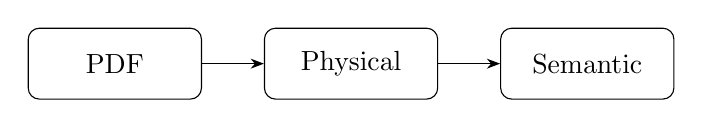
\begin{tikzpicture}[
      box/.style={draw, rounded corners, minimum width=2.2cm, minimum height=0.9cm},
      >=Stealth
    ]
    \node[box] (pdf) at (0,0) {PDF};
    \node[box] (phys) at (3,0) {Physical};
    \node[box] (sem) at (6,0) {Semantic};
    \draw[->] (pdf) -- (phys);
    \draw[->] (phys) -- (sem);
  \end{tikzpicture}
  \caption{Simple vector figure for graphics extraction tests.}
\end{figure}

\end{document}
